\chapter{Overview}
In this chapter, we introduce basic information and define essential terminology from~the~field of~bioinformatics. We describe the problem of~gene tree reconciliation in~more details and present existing software for solving this problem.

\section{Background}
Every organism has its complete set of genetic information encoded in a genome. A~genome consists of~several DNA (deoxyribonucleic acid) molecules and contains all the~information, which are required for~the~organism to~function.

DNA is a long molecule composed of~two complementary strands. Each strand is made up of~four chemical bases: adenine, guanine, cytosine and thymine, and connected to its complementary strand by~pairing rules, where adenine is paired up with~thymine and cytosine is paired up with~guanine. Sequence of~these bases encodes the genetic information important for~building and maintaining an~organism. Specific parts of~DNA are called genes.

A gene is a subsequence of~a~DNA strand that contains information for~synthesis of~a~specific molecule, usually a~protein. It is basic unit of~heredity.

The DNA sequence of a gene can be altered by mutation. It is a process that allows small changes in~DNA of~organisms that refers to~differences between individuals within a~population. We will be working with two types of mutations: duplication and deletion.

Duplication is a~type of~mutation where one or more genes are copied and inserted to~some other position in~the same genome. A~duplicated gene sometimes develops a~new function \cite{doyon}. 

The opposite of~duplication is deletion (gene loss). It~is a~type of~mutation in~which some part of~DNA sequence containing a~gene is left~out from~the~genome during DNA replication or it~loses its function. 

Speciation is an~evolutionary process of~in~which a~single population evolves populations into~two distinct species. It can happen for~various reasons, for~example, when a~group separates from~other members of~its species to~different a~geographical area. Members of~a~new group develop own unique characteristics due to~the~demands of~another environment and this process will differentiate the~new species.

Duplications and speciations result in formation of groups of~similar genes, called gene families, from a~single gene. A~gene family consists of~evolutionarily related genes from one or multiple species, which are structurally and usually functionally similar.

Evolutionary relationships formed by~evolutionary events are represented in~a~form of~graph called phylogenetic tree, which is a~branching diagram that~shows evolutionary relationships between organisms. A~phylogenetic tree is a~tree~$T$ with nodes~$V(T)$, edges~$E(T)$ and leaves~$L(T)$. It is called weighted when branch length~$w(u, v)$ is defined for~each edge~$(u, v)$.

Phylogenetic trees can be either rooted or unrooted (Fig. \ref{unrooted_rooted}). A~rooted tree is a~phylogenetic tree $T$ where for $(u, v) \in E(T)$: node $u$ is the parent of node $v$, node $v$ is the children of node $u$, $root(T)$ does not have parent and leaves $L(T)$ do not have children. An ancestor of node $v$ is any node of tree $T$ on the path from node $v$ to $root(T)$. Every ancestor have at least one descendant. An descendant of node $v$ is any node of tree $T$ of which $v$ is an ancestor \cite{hasic}. We will denote for $u, v \in V(T)$ that $v<_Tu$ if~$u$ is ancestor of~$v$ and $v$ is descendant of~$u$.

For~group of~nodes in~a~rooted tree, their~lowest common ancestor~(LCA) is the~farthest node from root that has all nodes in~the~group as~descendants.

An~unrooted tree is a~phylogenetic tree without root. Unrooted tree can be rooted by~placing a~root $r$ on some edge $(u, v)$. The~original edge $(u, v)$ is subdivided into two edges $(u, r)$ and $(r, v)$. If~edge $(u, v)$ is weighted, then $w(u, r) + w(r, v) = w(u, v)$.

\begin{figure}[h]
	\centering
	\label{unrooted_rooted}
  	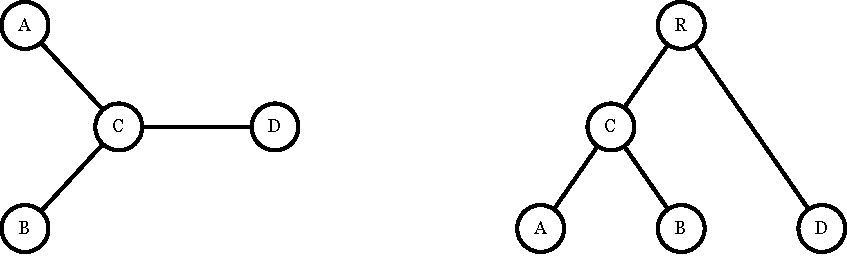
\includegraphics[width=\linewidth]{unrooted_rooted}
  	\caption{Unrooted tree(left) and its~rooted version (right) tree. We~placed the~root~$R$ on~the~edge~$(C, D)$ replacing it with~two new edges~$(C, R)$ and~$(R, D)$.}
\end{figure}

We will be using two types of phylogenetics trees for showing evolutionary relationships: species trees (to describe the~evolution of~a~set of~species) and gene trees (to describe evolution of~a~particular gene).

A~species tree is a~phylogenetic tree $S$ where $L(S)$ represent present-day species and internal nodes from $V(S)$ represent speciation events in~the~history.

A~gene tree is a~phylogenetic tree $G$ where $L(G)$ represent present-day copies of~the~gene and internal nodes from $V(S)$ represent duplication and deletion events in~the~history.

Phylogenetic trees are reconstructed from a multiple alignment of the DNA sequences of present-day species by various methods \cite{felsenstein} to find  the most likely phylogenetic tree to given DNA sequences.

\section{Different approaches to gene tree reconciliation}
An evolutionary history is a possible sequence of~evolutionary events that lead to~an~observed members of~a~gene family in~present-day species is shown by~evolutionary history (Fig. \ref{reconciliation}). It illustrates how many duplications and deletions happened during an~evolution of~one or more genes inside the evolution of~a~group of~species.

The~problem of~gene tree and species tree reconciliation was introduced in~1979 by~Goodman~et~al.~\cite{goodman} as~a~method to~infer evolutionary history of~duplications and deletions in~a~gene family to~decode evolutionary relationships between copies of~gene. The goal of~reconciliation consists in~mapping nodes of a gene tree into a species tree and thus inducing evolution of~a gene family in~terms of~speciations, duplications and deletions. An important prerequisite for~reconciliation is to~have a~gene tree without errors as~a~misplaced leaves can lead to~a different history of~the gene family.

\begin{definition}
A reconciliation between gene tree $G$ and species tree $S$ is mapping $\phi: V(G) \rightarrow V(S)$ such that:
	\begin{enumerate}\itemsep0em
	\item $\forall u \in L(G): \phi(u) = \mu(u)$
	\item $\forall u, v \in V(G)$ such that $v<_Gu$: $\phi(v)<_S\phi(u)$
	\end{enumerate}
	\label{def_reconciliation}
\end{definition}

An example of gene tree reconciliation is shown in Figure \ref{reconciliation}. We are given the gene tree $G$, the species tree $S$ and a leaf mapping $\mu: L(G) \rightarrow L(S)$ that maps each leaf from $G$ to leaf of its species in $S$. We will map internal nodes according to the second condition in Definition \ref{def_reconciliation}. Node $d$ is mapped to node $Y$, because it has $\phi(d)$ and $\phi(c)$ as descendants. It cannot be mapped to node $X$ since node $X$ does not have $\phi(c)$ as descendant thus $\phi(c)<_S\phi(d)$ would not hold. Then node $e$ is mapped above node $Y$ to have $\phi(a)$ and $\phi(d)$ as descendants. 

\begin{figure}[h]
	\centering
	\label{reconciliation}
  	\includegraphics[width=\linewidth]{reconciliation}
  	\caption{Reconciliation and evolutionary history. On~the~left, the~gene tree~$G$ is mapped to~the~species tree~$S$. On~the~right, we~can see the evolutionary history implied by this reconciliation. This~history contains one~duplication $e$, two speciations $Y$ and $X$ and three deletions (empty circles).}
\end{figure}

The LCA-mapping $\sigma: V(G) \rightarrow V(S)$ maps each node $u \in V(G)$ as low as possible to~the~unique node $\sigma(u) = LCA(\mu(v) | \forall v \in L(G), v<_Gu)$ in $S$. It satisfy both conditions in Definition \ref{def_reconciliation} and minimize the number of duplications and deletions. This reconciliation can be found in linear time \cite{hasic}.

Different approaches to~gene tree reconciliation will be shown with~presented examples of~software that have implemented gene tree reconciliation. 


\subsection{Scoring gene tree reconciliation}
Several software for gene tree reconciliation are known such as TreeBeST~\cite{treebest}, TreeFix~\cite{treefix} or Notung~\cite{notung}. 

TreeBest takes an unrooted gene tree, a rooted species tree and multiple sequence alignment for the gene family as input. They used method to create a tree with a model to penalize duplications and deletions relative to a known species tree. This program tends to produce duplication when the gene tree has extensive extant members on each side of the duplication.

TreeFix takes a rooted gene tree, a rooted species tree and multiple sequence alignment for the gene family as input. It creates mapping of gene tree leaves to species tree leaves from the alignment of sequences. It infers duplications and deletions using maximum parsimony reconciliation with duplication-deletion cost function, which looks for the reconciliation with minimum total number of duplications and deletions. Duplication ($D$) and deletion ($L$) have their costs ($c_D$ and $c_L$) that are set to one by default and can be changed by user. The duplication-deletion cost for one reconciliation can be written as: $c_D \cdot D+c_L \cdot L$. Same duplication deletion function is used by Notung.

Notung takes a rooted gene tree, a rooted species tree and the leaf mapping as input. If the gene tree is not rooted, it can be rooted by Notung rooting mode that gives each edge a root score (weighted sum of duplications and deletions). Apart from reconciliation of binary trees, Notung can reconcile binary gene trees with non-binary species trees and non-binary gene trees with binary species tree. Non-binary tree is a tree with at least one polytomy (a node with more than two children).
Reconciliation of binary gene trees to non-binary species trees results into binary gene tree. They use algorithm, that can distinguish between duplication and deep coalescence (divergence, when the time of separation of two  lineages precede the time of speciation) and leads to smaller total number of duplications and deletions than duplication-deletion cost function used in reconciliation of two binary trees \cite{vernot}. 
Reconciliation of non-binary gene tree to binary species tree results into non-binary gene tree. The general approach is to convert non-binary gene tree to binary gene tree that has minimal duplication-deletion score when reconciled with binary species tree. The resolution is then rearrange back to non-binary gene tree, where all nodes and edges not present in the original gene tree are removed and their assigned duplications and deletions are reassigned to their polytomy.

\subsection{Probabilistic gene tree reconciliation}
Probabilistic methods have been designed to~increase accuracy of~reconciled trees. Here, we~introduce two software tools that use probabilistic methods to~reconcile gene trees: SPIMAP and Phyldog.

SPIMAP software~\cite{spimap} reconciles a rooted gene tree in~the~presence of~a~known rooted species tree with given duplication and deletion rates that are estimated by Bayes approach. The~model infers duplication and deletion using the~birth-death process. The birth-death process is continuous-time process that generates a gene tree according to constant birth rate (representing duplication) and death rate (representing deletion). After running it for a time that represent branch length, all branches that exist at the time are "surviving" and others are "extinct". To initialize, they reconcile a single gene node to the root of $S$ and mark it as speciation. For every speciation, they run the birth-death process to generate a gene tree.

Another software is~PhylDog\cite{phyldog}, which uses method composed from~computing maximum likelihood of possible gene tree reconciliation to given species tree according to~duplication and deletion rates that are estimated for each branch separately. This model also uses the birth-death process, but birth and death rates are different for each branch.

They differ in~two aspects. First, while SPIMAP assumes duplication and deletion rates to~be~constant for~all branches in~the~species tree, PhylDog choose to~use particular pair of~duplication and deletion rates to~each branch of~the~species tree. Second, SPIMAP requires time-anchored species tree (branch length shows amount of~time between two nodes) to~compute likelihood of~a~gene family. Alternately, PhylDog calculate likelihood from~the~expected numbers of~duplications and deletions. 


\subsection{Isometric gene tree reconciliation}
Another variant of reconciliation is isometric gene tree reconciliation, where branch lengths are known and taken into~account while reconciling a gene tree and a species tree. The~branch length may express the expected number of substitution per site between two nodes. This~problem was introduced by~Ma~et~al.~\cite{ma} in~2008. They~presented an~algorithm with~$O(N^2)$ running time, where $N$ stands for~the~total number of~nodes in~the gene tree and the species tree. They~considered a rooted species tree and an unrooted gene tree, where both input trees have exact branch lengths.

This~algorithm was later corrected and modified by~Brejová~et~al.~\cite{brejova} to~an efficient algorithm with~$O(N \log N)$ running time. They also proposed two extensions of~the~problem. In~the~first extension, they considered both input trees (gene tree and species tree) unrooted and designed an~algorithm with~$O(N^5 \log N)$ running time. The second extension presents an~algorithm, where both input trees are rooted, but branch lengths are assumed to~be~scaled by~unknown scaling factor.

\begin{definition}
An isometric reconciliation between gene tree $G$ and species tree $S$ with branch lengths $w$, which are strictly positive, is mapping $\phi: V(G) \rightarrow V(S) \times R$ such that:
	\begin{enumerate}\itemsep0em
	\item $\forall u \in L(G): \phi(u) = [\mu(u), 0]$
	\item $\forall u, v \in V(G)$ such that $v<_Gu$: $\phi(v)<_S\phi(u)$ and $w(u, v) = d(\phi(u), \phi(v))$, where $d$ is the length of path between $u$ and $v$ in reconciled gene tree.
	\end{enumerate}
\end{definition}

\begin{figure}[h]
	\centering
	\label{isometric_reconciliation}
  	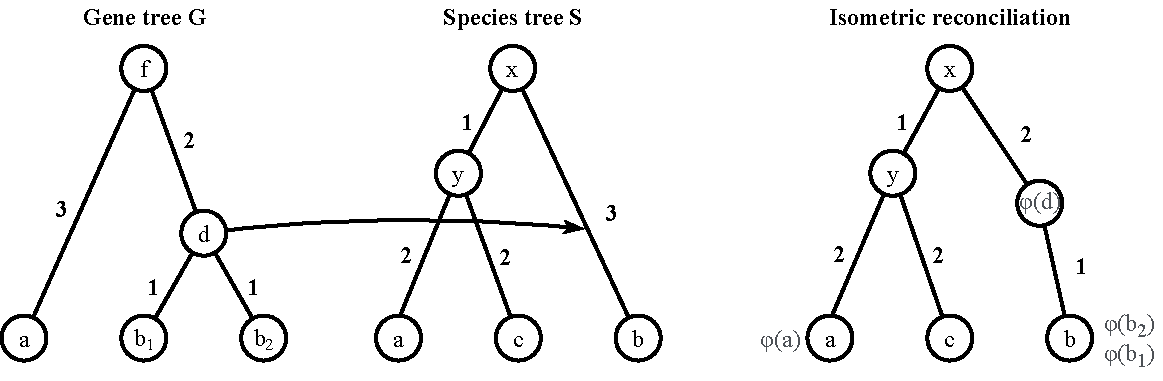
\includegraphics[width=\linewidth]{isometric_reconciliation}
  	\caption{Isometric reconciliation. On~the~left is mapping of~the~node~$d$ of~the~gene tree~$G$ to~the~edge~$(x, b)$ of~the~species tree~$S$. The result of~the~isometric reconciliation with~mapped node~$d$ is on~the~right.}
\end{figure}










